Let us denote \deftext{a mutual information} of three random variables:
$$
    I(\alpha : \beta : \gamma) \coloneqq I(\alpha : \beta) - I(\alpha : \beta \mid \gamma).
$$

The relations between quantities of information have a convenient geometric interpretation. Using Euler
diagrams, one can relate closed areas on the picture with quantities of information. For example, each
circle corresponds to an entropy of a random variable.

\begin{center}
    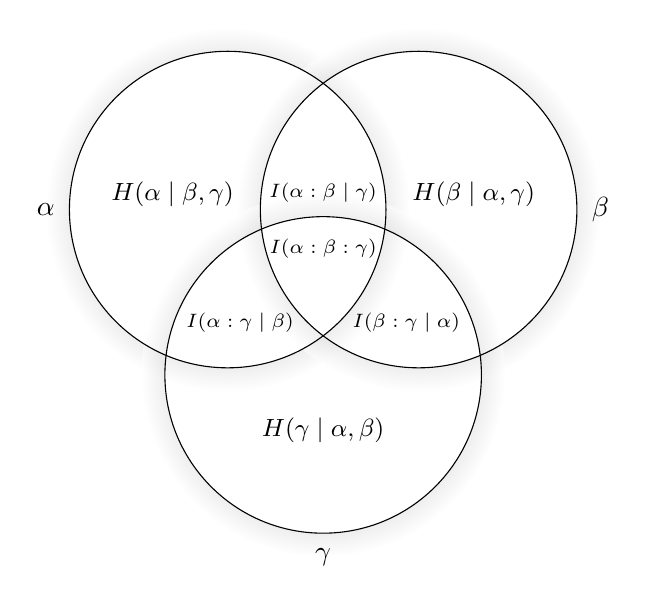
\begin{tikzpicture}
        \def\r{2.01}
        \def\R{1.4}

        \foreach \a in {150, 30, -90}{
            \shade[inner color = black, outer color = white, even odd rule, opacity = 0.5] (\a:\R)
                circle (\r + 0.3) circle (\r);
        }

        \draw (150:\R) circle (\r) node[shift = {(-\r - 0.3, 0)}] {$\alpha$};
        \draw (30:\R) circle (\r) node[shift = {(\r + 0.3, 0)}] {$\beta$};
        \draw (-90:\R) circle (\r) node[shift = {(0, -\r - 0.3)}] {$\gamma$};

        \node[shift = {(-0.7, 0.2)}] at (150:\R) {\small $H(\alpha \mid \beta, \gamma)$};
        \node[shift = {(0.7, 0.2)}] at (30:\R) {\small $H(\beta \mid \alpha, \gamma)$};
        \node[shift = {(0, -0.7)}] at (-90:\R) {\small $H(\gamma \mid \alpha, \beta)$};

        \node at (90:0.65 * \R) {\scriptsize $I(\alpha : \beta \mid \gamma)$};
        \node at (-35:0.92 * \R) {\scriptsize $I(\beta : \gamma \mid \alpha)$};
        \node at (215:0.92 * \R) {\scriptsize $I(\alpha : \gamma \mid \beta)$};

        \node at (0, 0.2) {\scriptsize $I(\alpha : \beta : \gamma)$};
    \end{tikzpicture}
\end{center}